

%use pdflatex

\documentclass[12pt]{amsart}
\usepackage[utf8]{inputenc}
\usepackage{url}
\usepackage{color}
\usepackage[margin=1in]{geometry}


\usepackage{tikz-cd}
\usepackage{mathtools}
\usetikzlibrary{matrix,arrows,decorations.pathmorphing}
\usepackage{amssymb,latexsym, amsmath, amsthm,pdfsync}
\usepackage{enumerate}
\usepackage{hyperref}
\usepackage{enumitem}
\usepackage{float}
\usepackage{tikz}
\usepackage{setspace}
\usepackage{arcs}
\usepackage[ruled, lined, linesnumbered, commentsnumbered, longend]{algorithm2e}
\usepackage{caption}
\usepackage{subcaption}
\usepackage[normalem]{ulem}
\DeclareMathOperator{\argmax}{argmax}
\DeclareMathOperator{\arcsec}{arcsec}


\makeatletter
\g@addto@macro{\@algocf@init}{\SetKwInOut{Parameter}{Parameters}}
\makeatother
%arc of a circle
\makeatletter
\DeclareFontFamily{U}{tipa}{}
\DeclareFontShape{U}{tipa}{m}{n}{<->tipa10}{}
\newcommand{\arc@char}{{\usefont{U}{tipa}{m}{n}\symbol{62}}}%

\newcommand{\arc}[1]{\mathpalette\arc@arc{#1}}

\newcommand{\arc@arc}[2]{%
\sbox0{$\m@th#1#2$}%
\vbox{
\hbox{\resizebox{\wd0}{\height}{\arc@char}}
\nointerlineskip
\box0
}%
}
\makeatother
\newlist{steps}{enumerate}{1}
\setlist[steps, 1]{label = Step \arabic*:}
\newlist{case}{enumerate}{1}
\setlist[case, 1]{label = Case \arabic*:}

\theoremstyle{plain}
\newtheorem{theorem}{Theorem}[section]
\newtheorem{corollary}[theorem]{Corollary}
\newtheorem{lemma}[theorem]{Lemma}
\newtheorem{proposition}[theorem]{Proposition}
\newtheorem{remark}[theorem]{Remark}
\newtheorem{conjecture}[theorem]{Conjecture}
% \theoremstyle{definition}
\newtheorem{definition}[theorem]{Definition}
 \newtheorem{question}[theorem]{Question}
\usetikzlibrary{positioning}
 \newtheorem{example}[theorem]{Example}

\tikzset{main node/.style={circle,fill=blue!20,draw,minimum size=0.5cm,inner sep=0pt},}

\definecolor{darkblue}{rgb}{0.0, 0.0, 0.8}
\definecolor{darkred}{rgb}{0.8, 0.0, 0.0}
\definecolor{darkgreen}{rgb}{0.0, 0.8, 0.0}


\newcommand{\Z}{\mathbb{Z}}
\newcommand{\Q}{\mathbb{Q}}
\newcommand{\R}{\mathbb{R}}
\newcommand{\C}{\mathbb{C}}
\newcommand{\Sp}{\mathbb{S}}
\newcommand{\diam}{\mathrm{diam}}
\newcommand{\dgh}{d_\mathrm{GH}}
\newcommand{\dH}{d_\mathrm{H}}
\newcommand{\homsing}{\mathrm{H}^\mathrm{s}}
\newcommand{\homsimp}{\mathrm{H}^\Delta}
\newcommand{\filrad}{\mathrm{FillRad}}
\newcommand{\sfilrad}{\mathrm{sFillRad}}
\newcommand{\hyp}{\mathrm{hyp}}
\newcommand{\rad}{\mathrm{rad}}
\newcommand{\spread}{\mathrm{spread}}
\newcommand{\h}{\mathrm{H}}
\newcommand{\mr}{\mathrm{MR}}
\newcommand{\vol}{\mathrm{vol}}


%% commands for dgms
\newcommand{\dgm}{\mathrm{barc}}
\newcommand{\dgmR}{\dgm^\mathrm{VR}}
\newcommand{\dgmRzero}{\mathrm{rbarc}^\mathrm{VR}}

%%%%%%%%%%%%%%%%%%%%

\newcommand{\Hom}{\mathrm{H}}
\newcommand{\PH}{\mathrm{PH}}
\newcommand{\vr}{\mathrm{VR}}
\newcommand{\per}{\mathrm{B_*}}
\newcommand{\met}{\mathrm{Met}}
\newcommand{\pmet}{\mathrm{PMet}}
\newcommand{\hpmet}{\mathrm{HPMet}}
\newcommand{\htop}{\mathrm{hTop}_*}
\newcommand{\betti}{\beta_1}
\newcommand{\db}{d_\mathrm{b}}
\newcommand{\dhi}{d_\mathrm{HI}}
\newcommand{\di}{d_\mathrm{I}}
\newcommand{\norm}[1]{\left\lVert#1\right\rVert_{L^\infty}}
\newcommand{\comax}{\mathrm{comax}}
\newcommand{\np}{Z}

\newcommand{\katz}[1]           {{ \textcolor{darkblue} {#1}}}
\newcommand{\qingsong}[1]   {{ \textcolor{darkblue} {#1}}}
\newcommand{\facundo}[1]     {{ \textcolor{darkred} {#1}}}


\numberwithin{equation}{section}



\title{Extremal spherical polytopes and Borsuk's conjecture}

\date{}


%\linespread{1.5}


\author{Mikhail  Katz}
\address{Bar Ilan University.}
\email{katzmik@math.biu.ac.il }

\author{Facundo M\'emoli}
\address{The Ohio State University.}
\email{facundo.memoli@gmail.com}


\author{Qingsong Wang}
\address{University of Utah.}
\email{qswang@math.utah.edu}
\begin{document}



\maketitle



\begin{abstract}
We generate anti-self-polar polytopes via a numerical implementation of the gradient flow induced by the diameter functional on the space of all finite subsets of the sphere, and prove related results on the critical points of the diameter functional as well as results about the combinatorics of such polytopes. We also discuss potential connections to Borsuk's conjecture.

\end{abstract}


\tableofcontents

\section{Introduction}



Let $(X, d_X)$ be a metric space.  The \emph{Kuratowski embedding} $x
\mapsto d_X(x, \cdot)$ is an embedding of $X$ into $L^{\infty}(X)$,
the space of all bounded real-valued functions on $X$ with the uniform
norm.  When $X$ is the unit sphere with its geodesic distance, the
homotopy types of the $r$-neighborhoods $B_r(X, L^{\infty}(X))$ in the
Kuratowski embedding of $X$ were studied by Katz
in~\cite{katz1991neighborhoods}.  The values at which the homotopy
type changes are closely related to the critical configurations of the
diameter functional $\diam$ of $X$ which maps a finite subset $A$ of
$X$ to $\diam(A):=\max_{a,a'\in A}d_X(a,a')$.  When $X$ is the unit
circle, such critical values turn out to be exactly one-half of the
diameter values of odd regular polygons inscribed in $\Sp^1$.  Note
that the vertex sets of odd regular polygons are exactly the
configurations that are local minima of the diameter functional on the
{space of all finite subsets of $\Sp^1$ equipped with Hausdorff
  distance}.  In \cite{katz1989diameter}, Katz studied the
diameter-extremal configurations on $\Sp^2$ and $\Sp^3$.  The latter
provide candidates for testing Borsuk's conjecture in $\R^4$ (see
below).

Recently, Lim, M\'{e}moli, and Okutan
\cite[Theorem~5]{lim2020vietoris} proved that the homotopy types of
neighborhoods of the Kuratowski embedding of $X$ are naturally
homotopy equivalent to the so-called \emph{Vietoris--Rips complexes}
of $X$, a central object in the field of applied algebraic topology.
Therefore, the study of diameter-extremal configurations is also of
interest for understanding the properties of the Vietoris-Rips complex
of spheres \cite{adams-s1,adams-ot}.

In this paper, we extend the investigation of diameter-extremal
configurations on spheres started in~\cite{katz1989diameter}.  In the
$\Sp^1$ case, the critical values of the diameter functional form a
convergent sequence with the only accumulation point being $\pi$.  It
is natural to wonder to what extent a similar behavior is true on
$\Sp^2$.  We consider two canonical families of diameter-extremal
configurations on $\Sp^2$ which we call pyramids $A_k$ that contains
$2k+2$ points (see Section~\ref{subsec:pyramid_config}) and
stacked-triangles $B_k$ that contains $3k+1$ points (see
Section~\ref{subsec:stack_config}).  Both families contain infinitely
many members with diameters monotonically approaching
$\frac{2\pi}{3}$.  We prove in
Theorem~\ref{thm:finiteness_of_minimal_configurations} that
$\frac{2\pi}{3}$ is in fact the first accumulation point of the set of
critical values of the diameter functional.  In Proposition~\ref{p17},
we prove that the two families $A_k$ and $B_k$ do not exhaust all the
possible configurations with similar diameter bounds, and in fact
there are infinitely many additional diameter-extremal configurations.
Diameter-extremal configuration with $3k$ points can be found by
performing diameter gradient flow on a certain subset of $B_k$.  When
$k$ is odd, by a parity argument, the resulting configuration cannot
be an instance of $A_k$ or $B_k$.

We next devise and implement a computational algorithm (see
Algorithm~\ref{alg:diameter_gradient_flow}) that attempts to produce
diameter extremal configurations.  We use this algorithm to find new
configurations not in $A_k$ or $B_k$.  Furthermore, we found
configurations not isometric to the ones produced in the course of
proving Proposition~\ref{p17}.  See Table~\ref{tbl:pointwise extremal
  configurations_S2} for a complete list of all the configurations we
found in this way with up to 10 points. The list contains
  $10$ previously unknown configurations where $8$ of those exhibit
  $\mathbb{Z}_2$ symmetry and the remaining two are asymmetric; see
  Figures~\ref{figure:C_diam_graph} and~\ref{figure:D_diam_graph}.

The convex hulls of certain diameter-extremal configurations give rise
to \emph{anti-self-polar polytopes} (ASP), for example, the regular
tetrahedron and any $A_k$ or $B_k$.  ASPs are polytopes $P$
characterized by the property that the polar of $P$ equals $-P$ (see
Definition \ref{defn:asp}).  ASPs have been studied by Lov\'{a}sz in
the context of answering a question by Erd\"os and Graham
\cite{lovasz1983self} and were also considered in \cite[Section
  5]{katz1989diameter} in the context of Borsuk's conjecture.


 Borsuk's conjecture (see Section~\ref{subsec:Borsuk_conjecture}) for
 a finite point set $X$ in $\R^n$ is equivalent to the property that
 the chromatic number of the diameter graph (see Definition
 \ref{defn:diam_graph}) of $X$ is bounded above by $n+1$.  We continue
 to explore the suggestion in \cite{katz1989diameter} to use
 diameter-extremal configurations on $\Sp^3$ to test Borsuk's
 conjecture in $\R^4$ (a case that is still open).  As shown by Lovasz
 \cite{lovasz1983self}, the chromatic number of the diameter graph
 associated to any ASP in $\R^n$ is at least $n+1$.  An ASP for which
 the inequality is strict would disprove Borsuk's conjecture.

It was conjectured in \cite{katz1989diameter} that the number of edges
in the diameter graph of an ASP $4$-polytope with $v$ vertices is at
least $3v-5$.  We use Kalai's inequality from \cite[Section~4.3]{Ka94}
to prove such a bound in Theorem~\ref{thm:num_edges_S_3} below.
We then formulate conjectures about the number of edges in
  the diameter graph for more general subsets on $\Sp^3$, see
  Conjectures~\ref{conj:num_edges_S_3} and \ref{conj:3x-5}.  A
  calculation based on these two conjectures suggests that the maximum
  possible chromatic number of the diameter graph of a finite subset
  $X\subseteq \R^4$ is $6$ instead $5$, the number predicted by
  Borsuk's conjecture.
%

We perform experiments attempting to identify diameter-extremal
configurations on the three-dimensional sphere.  The interest in these
experiments is twofold.  On the one hand, it is naturally interesting
to obtain an understanding of critical configurations beyond the case
of $\Sp^1$ and $\Sp^2$.  On the other hand, whereas Borsuk's
conjecture is known to be true in dimensions $2$ and $3$ but false in
dimensions $64$ and higher, its status for dimension $4$ is unknown.
Hence, by the above, it is tempting to seek a diameter-extremal
configuration $X$ of $\Sp^3$ whose convex hull is an ASP such that its
diameter graph has chromatic number at least $6$.
We discovered 65 new configurations on $\Sp^3$ not obtained
  by the pyramid construction (see~\ref{subsec:pyramid_config}) on a
  previously known configuration on $\Sp^2$; see Theorem~\ref{t61}.
However, all the diameter graphs of these configurations have a
chromatic number precisely~$5$.%

\medskip

\noindent
\textbf{Acknowledgements.} This work was partially supported by BSF \#2020124, NSF CCF \#1740761, NSF CCF \#1839358 and NSF IIS \#1901360.



\section{Pointwise extremal sets}


Let $\Sp^n\subseteq\R^{n+1}$ be the unit sphere with its geodesic
distance.  For a subset $Y\subseteq\Sp^n$, its diameter $\diam(Y)$ is
computed with respect to the geodesic distance on the sphere.

\begin{definition}[Taut sets in $\Sp^n$]
A finite subset $Y\subset \Sp^n$ is \emph{taut} if one of the
following equivalent conditions is satisfied:
\begin{enumerate}
\item
the convex hull of $Y$ contains the origin;
\item
there are non-negative real numbers $\{a_y\}_{y\in Y}$, not all zero,
satisfying
\[
\sum_{y\in Y}{a_y \, y} = 0,
\]
where $y$ denotes the position vector of the point $y\in \R^{n+1}$.
\end{enumerate}
\end{definition}



	 Jung's theorem immediately gives the following result.
	\begin{proposition}\label{prop:Jung}
		If $Y\subset \Sp^{n}$ is taut, then $\diam(Y)\geq \arccos\left(\frac{-1}{n+1}\right)$.
	\end{proposition}



The following observation will be useful in the sequel.



	\begin{corollary}\label{coro:taut_positive_coeff}
Let $Y \subset \Sp^n$ be a taut set such that $|Y|=n+2$ and
$\diam(Y)<\arccos\left(-\frac{1}{n}\right)$.  Then the dimension of
the vector space spanned by $Y$ is equal to $n+1$.\\ In particular, if
$\{a_1,\ldots,a_{n+2}\}$ is any set of non-negative coefficients such
that
		\[
	\sum_{i=1}^{n+2}\,{a_i y_i} = 0,
		\]
		then all $a_i$ must be positive.
	\end{corollary}
	\begin{proof}
		% Suppose the above conclusion is false and without loss of generality, we may assume $a_{n+2} = 0$.
		% Then the set of vectors $\{y_1, y_2, \cdots, y_{n+1}\}$ is linearly dependent.
%
Suppose the vector space spanned by all points in $Y$ is of dimension
at most $n$. Then, the set $\{y_1, y_2, \ldots, y_{n+2}\}$ must lie on
some great sphere $\Sp^{n-1}\subseteq\Sp^n$ and it must be taut in
$\Sp^{n-1}$.  Then, by Proposition~\ref{prop:Jung}, the set $Y$ must
have diameter at least $\arccos\left(-\frac{1}{n}\right)$ which
contradicts the assumptions on $Y$. This concludes the first part of
the proof.\\ For the second part, without loss of generality, we
assume that $a_1 = 0$, then the set of vectors $\{y_2, y_3 \ldots,
y_{n+2}\}$ is linearly dependent and hence
$\mathrm{dim}(\mathrm{span}\{y_2, y_3, \ldots, y_{n+2}\}) < n+1$.  The
contradiction with the first part establishes the result.
	\end{proof}




Let $Y$ be a subset of a metric space $(X, d_X)$.  For any two points
$y, y'\in Y$, we say that $y$ and $y'$ are \emph{comaximal} in $Y$ if
$d_X(y, y') = \diam(Y)$.  In such a case, $y$ is called a
\emph{comaximal point} with $y'$.  We use the notation
$\comax_Y^{\phantom{I}}(y)$ to denote the set of all points in $Y$
which are comaximal with $y$.

For two points $x, x'\in \Sp^n$ with distance less than $\pi$, there
is a unique arclength-parametrized geodesic $\gamma_{x,x'}$ connecting
$x$ to $x'$ such that $\gamma_{x,x'}(0)=x$.  Consider the \emph{unit}
tangent vector $\dot{\gamma}_{x,x'}(0)$ in the tangent space
$T_x\Sp^n$.

We recall the notion of \emph{pointwise extremal subsets} in $\Sp^n$
as in \cite{katz1989diameter}.


\begin{definition}[\cite{katz1989diameter}]\label{defn:pointwise_extremal}
Let $Y\subseteq\Sp^n$ be a \emph{finite} subset with no antipodal
pairs.  We say that $y\in Y$ is \emph{held} (in place) by $Y$ if the
set of vectors $\dot{\gamma}_{y,y'}(0)$ as $y'$ runs over
$\comax_Y^{\phantom{I}}(y)$ is a taut set.  We say that $Y$ is
\emph{pointwise extremal} if every point $y\in Y$ is held by $Y$.
\end{definition}

When $n=1$, it is not difficult to see that, for all integers $k\geq
1$, the vertex set of an inscribed regular $(2k+1)$-gon is pointwise
extremal.  The following proposition shows the converse.


\begin{proposition}\label{prop:one_dim_pointwise extremal configurations_is_odd_gon}
Let $Y\subseteq \Sp^1$ be a pointwise extremal set containing no pair
of antipodal points.  Then $Y$ is the vertex set of an odd regular
polygon inscribed in $\Sp^1$.
\end{proposition}


\begin{proof}
Let $y\in Y$ and let $D=\diam (Y)$.  Let $R_D$ be the clockwise rotation
on $\Sp^1$ by angle~$D$.  As $y$ is held by $Y\subseteq \Sp^1$, the
set $Y$ must contain both points in $\Sp^1$ at distance $D$ from $y$.
In particular, the set $Y$ is invariant under the rotation $R_D$.  As
$Y$ is a finite subset, the quotient $\frac{D}{2\pi}$ must be
rational.  Let $\frac{m}{n}$ be the representation of $\frac{D}{2\pi}$
in lowest terms.  Then the orbit of $y$ under the rotation $R_D$ forms
the vertex set of an inscribed regular $n$-gon $Y'\subseteq\Sp^1$.  As
$Y$ does not contain any antipodal pairs, $n$ is necessarily odd.
Therefore, $Y$ contains the vertex set of a odd regular $n$-gon $Y'$
of the same diameter as $Y$.  Then $Y$ must coincide with $Y'$ as
adding any additional point to the set $Y'$ would strictly increase
the diameter.
\end{proof}

\subsection{The  pyramid construction}\label{subsec:pyramid_config}
In this section, we describe a class of pointwise extremal subsets of
$\Sp^n$ called \emph{pyramids} in \cite{katz1989diameter}. For any
pointwise extremal subset $Y\subset \Sp^{n-1}$, the pyramid
construction provides a corresponding pointwise extremal subset in
$\Sp^n$ that consists of a rescaled copy of $Y$ together with one
extra point.  Let $\Sp^n\subseteq\R^{n+1}$ be the unit sphere.
Let~$\np=(0,\dots,0,1)$ denote the ``north pole''.  Let $x_{n+1}$ be
the last coordinate of $\R^{n+1}$. Then for each plane \{$x_{n+1} =
a\}, a\in \R$ that meets $\Sp^n$ at more than one point, the
intersection is a rescaled copy of $\Sp^{n-1}$ which we call a
\emph{horizontal section}.  Each horizontal section contains a
suitable rescaled copy of $Y$ which is isometrically embedded into it.

\begin{definition}
The \emph{pyramid over $Y$} is the subset of $\Sp^n$ consisting of the
north pole $\np$ together with a rescaled copy $Y'$ of $Y$ inside some
horizontal section such that the diameter of $Y'$ equals the distance
from $\np$ to the horizontal section.  Denote by $\mathrm{Pyr}(Y)$ the
pyramid over a pointwise extremal subset $Y$.
\end{definition}

Let $x,y\in Y$ be points with $d_{\Sp^{n-1}}(x, y) = \diam(Y)$.  Let
$x', y'\in\mathrm{Pyr}(Y)$ be points corresponding to $x,y$.
Then the triple $\np, x', y'$ is the vertex set of a spherical
equilateral triangle, with spherical angle $\sphericalangle\,x'\np
y'=\diam(Y)$.  Applying the spherical theorem of cosines to the
geodesic triangle $\triangle\,x'\np y'$, we obtain the following
relationship:
$$\diam(\mathrm{Pyr}(Y)) = \arcsec\left(\sec\big(\diam(Y)\big)-1\right).$$


\begin{example}[The $A_k$ family in $\Sp^2$]\label{example:A_k}
Let $k\geq1$.  We apply the pyramid construction to the regular
$(2k+1)$-gon on $\Sp^1$ to obtain a pointwise extremal configuration
$A_k \subseteq \Sp^2$, consisting of the north pole of $\Sp^2$
together with a suitably rescaled copy of the regular $(2k+1)$-gon, so
that $\diam
(A_k)=\arcsec\left(\sec\big(\frac{2k\pi}{2k+1}\big)-1\right)$; see
Figure \ref{fig:penta-pyr}.  In particular, the
  diameter $\diam(A_k)$ tends to $\frac{2\pi}{3}$ as $k$ goes to
  infinity.
\end{example}

\begin{figure}[H]
	\centering
	\includegraphics[scale=0.4]{./figures/small_A2.pdf}
	\caption{The configuration $A_2$ consists of the north pole and the vertices of a regular pentagon. }\label{fig:penta-pyr}
\end{figure}


\subsection{Construction of $k$-stacks}\label{subsec:stack_config}

Following~\cite{katz1989diameter}, let a $\beta$-\emph{digon} be the
convex region on $\Sp^2$ bounded by two meridians (great semicircles
joining the north and south poles), with angle $\beta$ between the two
meridians.

Given a $\beta$-digon, we now introduce a procedure that will be used
to produce a certain type of pointwise extremal set $Y\subseteq \Sp^n$
called a $k$-\emph{stack}. The \emph{digon procedure} is a ``walking
process" on the digon that takes as input an odd integer $2k + 1
\geq3$ and outputs a suitable step length $d_1 > \beta$.

We start walking with equal steps from the north pole on alternating sides of the digon, with step length $d_1$ calibrated so as to get exactly to the south pole after $2k+1$ steps; see Figure~\ref{fig:eqs}.

Let $\np\in\Sp^n$ be the north pole.  A regular $n$-simplex inscribed
in the equator $\Sp^{n-1}\subset\Sp^{n}$ defines $n+1$ meridians
passing through the vertices of the simplex.

Let $\ell \in (0, \pi)$.  The set of points on $\Sp^n$ which are at
distance $\ell$ away from the north pole $\np$ is a rescaled
$(n-1)$-sphere $\Sp_\ell^{n-1}$, namely a horizontal section of
$\Sp^n$.  The intersection between $\Sp_\ell^{n-1}$ and the set of
$n+1$ meridians is the vertex set of an inscribed $n$-simplex in
$\Sp_\ell^{n-1}$.


Let $k\geq1$.  A $k$-stacked configuration $Y$ (see Figure
\ref{fig:eqs}) consists of the north pole $\np$ together with the
union of the vertex sets of $k$ stacked $n$-simplices each obtained as
the intersection of a horizontal $(n-1)$-sphere $\Sp^{n-1}_{\ell_i}$
with the $n+1$ meridians. The distances $\ell_1,\ldots,\ell_k$ between
the horizontal sections and the north pole are determined by the digon
procedure as follows.  Let $d_1$ be the step length that comes from
the digon procedure with input $2k+1$.  Consider the sequence of
numbers $\{d_j\}_{j=0}^{2k+1}$ where $d_j$ is the distance to the
north pole of the point obtained after walking $j$ steps in via the
digon procedure.  Then, the sequence of numbers $\{\ell_{i}\}_{1\leq i
  \leq k}$ is defined in terms of $\{d_i\}_{i=0}^{2k+1}$
by setting
\[
\ell_i=d_{2i} \quad \text{for} \quad 1\leq i\leq k.
\]
Note that $d_{2k}=\diam(Y)$ and $d_{1} = \pi - d_{2k}$.


Given an odd integer $2k+1\geq 3$, the following system of equations summarizes the computation of $d_i$ for $1\leq i\leq  2k+1$.



Let $\beta_n= \arccos(\frac{1}{n})$. The values $\{d_i\}_{0\leq i\leq
  2k+1}$ are determined by $n$ and $k$ via the following equations
(see Figure \ref{fig:eqs}):
\begin{equation}\label{eqn:digon}
	\begin{cases}
		d_0 = 0, \; d_{2k+1} = \pi                                                               \\
		\cos(d_i)\cos(d_{i+1}) + \sin(d_i)\sin(d_{i+1})\cos(\beta_n) = \cos(d_1), \,\,1\leq i \leq 2k \\
		d_i + d_{2k+ 1 - i} = \pi, \,\,0\leq i \leq 2k + 1.
	\end{cases}
\end{equation}


\begin{remark}
Let $d_1$ be the output of the digon procedure with input $2k+1$ on a
digon of angle $\beta$.  If we perform the ``walking process'' on a
digon of angle $\pi-\beta$ with complementary step length $\pi - d_1$,
we will eventually get close to the south pole (but will not reach it)
and then will start walking back to the north pole and reach it after
$2k+1$ steps. If we add an edge between the points that we traveled
during the ``walking process'', we obtain the diameter graph (see Definition~\ref{defn:diam_graph}) of a
regular $2k+1$-gon.
\end{remark}
\begin{figure}
    \centering
    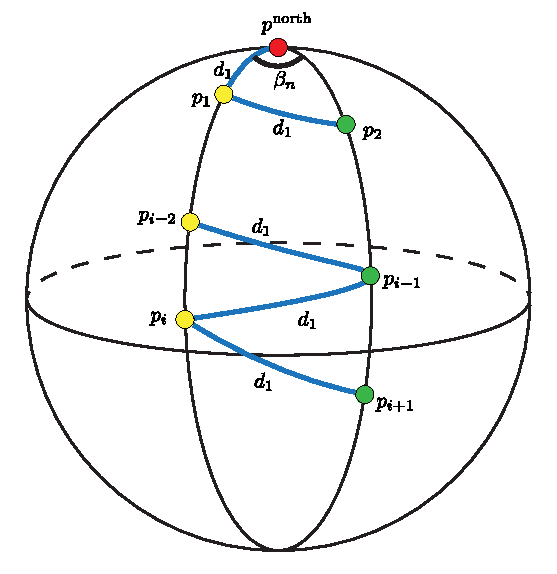
\includegraphics[scale=0.75]{./figures/digon.pdf}
    \caption{Each value $d_i$ in Equation~(\ref{eqn:digon}) is the distance between the point  $p_i$ shown in this figure and the north pole.
		For  $1\leq i\leq 2k+1$, the distance between $p_i$ and $p_{i+1}$ is $d_1$.
		The two conditions in Equation~(\ref{eqn:digon}) are obtained by requiring $p_0$ to be the north pole and $p_{2k+1}$ to be the south pole.
		The conditions in the second line of Equation~(\ref{eqn:digon}) are obtained by applying the theorem of cosines for the geodesic spherical triangles with vertices $\{\np,\,p_i,\,p_{i+1}\}$, for each $1\leq i \leq 2k+1$.
		The third line  Equations (\ref{eqn:digon}) is obtained by symmetry considerations.}
    \label{fig:eqs}
\end{figure}


\begin{example}[The $B_k$ family in $\Sp^2$]\label{example:B_k}
When $n=2$, for each $k$, we denote the stacks that result from the
digon procedure by $B_k$, which consists of the vertices of $k$
stacked triangles ($2$-simplices) together with the north pole. Note
that $B_1$ coincides with the configuration $A_1$ from
Example~\ref{example:A_k}.  By construction,
  $\diam(B_k) = \pi - d_1 < \pi - \arccos(\frac{1}{2}) =
  \frac{2\pi}{3}$ and $\lim_{k\rightarrow \infty} \diam(B_k) =
  \frac{2\pi}{3}$.
\end{example}

	
	

\begin{figure}[H]
	\centering
	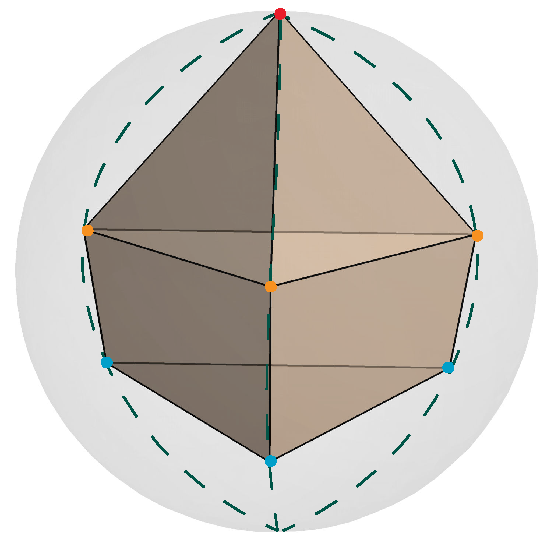
\includegraphics[scale=0.4]{./figures/small_B2.pdf}
	\caption{The configuration $B_2$ that consists of the north pole and vertices of two stacked triangles. The green dash lines are meridians; the red dot is the north pole, and points of the same color are of the same distance to the north pole.}
\end{figure}

\begin{example}[The $T_k$ family in $\Sp^3$]\label{example:T_k}
Let $n=3$.  For each $k$, we denote the stacks that result from the
digon procedure by $T_k$, which consists of the vertices of $k$
stacked tetrahedra together with the north pole.
\end{example}


\section
{Minimal sets on $\Sp^2$ with diameter below the first accumulation
  critical value}

Let $d>0$ and let $\mathcal D(\Sp^2, d)$ be the set of all finite
subsets $Y\subset \Sp^2$ with $\diam(Y)<d$.

As each finite subset on $\Sp^2$ is closed, the Hausdorff distance $\dH$ is a metric on $\mathcal D(\Sp^2, d)$.

\begin{definition}
[Diameter-extremal sets in $\mathcal D(\Sp^2,
  d)$~\cite{katz1989diameter}] A subset $Y\in \mathcal D(\Sp^2, d)$ is
called \emph{diameter-extremal} for the diameter functional if there
is a little-$o$ function such that
	\[
	\diam(Y) \leq \diam(Y') + o(\,\dH(Y, Y'))
	\]
	for all $Y'\subset \Sp^2$.
    In other words, we have
	\[
		\lim_{\dH(Y', Y) \rightarrow 0}\frac{\diam(Y')-\diam(Y)}{\dH(Y', Y)}\geq 0.
	\]

\end{definition}

\begin{remark}
An $n$-point set $Y$ is diameter-extremal if and only if at the
corresponding point in the configuration space $(S^2)^{\times n}$, the
gradients of the distances between pairs of points at maximal distance
form a taut set (see further in Section~\ref{s31}).
\end{remark}

\begin{lemma}
[{\cite[Corollary~3.4]{katz1989diameter}}]
\label{lem:critical_is_pointwise_extremal}
A diameter-extremal set $Y\in \mathcal D(\Sp^2, \frac{2\pi}{3})$ is
necessarily pointwise extremal.
\end{lemma}


\begin{definition}
[Minimal set in $\mathcal D(\Sp^2, d)$~\cite{katz1989diameter}] A
subset $Y\in \mathcal D(\Sp^2, d)$ is called a \emph{minimal set} if
there is some $\delta>0$ such that $\diam(Y)\leq \diam(Y')$ for all
finite subsets $Y'$ with $\dH(Y, Y')\leq \delta$.
\end{definition}

Clearly, every minimal set is diameter-extremal.  In fact, there is a converse.

\begin{theorem}[
{\cite[Theorem 2]{katz1989diameter}}]\label{thm:critical_is_minimal}
  Every diameter-extremal set in $\mathcal D(\Sp^2, \frac{2\pi}{3})$
  is a minimal set on $\Sp^2$.
\end{theorem}

By a mountain-pass argument, one obtains the following consequence.

\begin{lemma}
[{\cite[Corollary
      2]{katz1989diameter}}]
\label{lem:unique_minimal_in_connected_component}
There is exactly one (up to congruence) minimal set in each connected
component of $\mathcal D(\Sp^2, \frac{2\pi}{3})$.
\end{lemma}


\subsection{Configuration space}
\label{s31}

We will now estimate the number of such connected components.  We use
the notation $\prod\limits_{\diam \leq d}^k\Sp^2$ to denote the set of
all tuples $(y_1, \dots, y_k)$ in $\prod^k \Sp^2$ such that the
diameter of its associated set $\{y_1, \dots, y_k\}$ is less than or
equal to $d$.  Note that, for any $\epsilon>0$, we have a natural
continuous map
\[
	\prod\limits_{\diam \leq d}^k\Sp^2 \longrightarrow \mathcal
        D(\Sp^2, d + \epsilon).
\]
By realizing $\prod\limits_{\diam \leq d}^k\Sp^2$ as a closed
semi-algebraic set, we obtain the following upper bound on the number
of connected components in $\prod\limits_{\diam \leq d}^k\Sp^2$.


\begin{lemma}\label{lem:finiteness_of_connected_components}
Let $k\geq0$.  We set $s_k= 2k + \frac{k(k+1)}{2}$.  Then, for every
$d>0$, the number $b_0(k,d)$ of connected components of
$\prod\limits_{\diam \leq d}^k\Sp^2$ satisfies
$$ b_0(k,d)\leq 2s_k(4s_k-1)^{3k-1}.$$
\end{lemma}

\begin{proof}
	We will first describe the set $\prod\limits_{\diam \leq d}^k\Sp^2$ as a closed basic semi-algebraic set in $\R^{3k}$.
	Let $x_{i, j}$, where $1\leq i\leq k$ and $1\leq j\leq 3$, denote the standard coordinates in $\R^{3k}$. Then the set $\prod\limits_{\diam \leq d}^k\Sp^2$ is characterized by the following conditions:
	\begin{equation*}\label{eqn:semi_alg}
		\begin{cases}
			x_{i, 1}^2 + x_{i, 2}^2 + x_{i, 3}^2  =  1\quad\text{for all $1\leq i\leq k$,}\\
			(x_{i, 1} - x_{i', 1})^2 + (x_{i, 2} - x_{i', 2})^2 + (x_{i, 3} - x_{i', 3})^2 \leq d^2 \quad\text{for all $1\leq i< i'\leq k$.}
		\end{cases}
	\end{equation*}
Therefore the set $\prod\limits_{\diam \leq d}^k\Sp^2$ is a basic
semi-algebraic set given by $s_k =2k + \frac{k(k+1)}{2}$ non-strict
inequalities.  Then Theorem~\ref{thm:bound_betti_basic_semi_alg}
implies that $ b_0(k,d)\leq \frac{1}{2}(2s_k+2)(2s_k+1)^{3k-1}.$
\end{proof}

\subsection{Finiteness results}


Lemma~4.1 and Lemma~4.3 in \cite{katz1989diameter} imply the following
result.

\begin{lemma}[{\cite{katz1989diameter}}]
Let $0<d<\frac{2\pi}{3}$.  Let $Y\in \mathcal D(\Sp^2, d)$ be a
pointwise extremal set.  Then for any pair of distinct points $y, y'$
in $Y$, the distance $d_{\Sp^2}(y, y')$ is at least $\arccos\left(
2\frac{\cos^2(d)}{\cos^2(d/2)}-1\right)$.
\end{lemma}

By a packing argument on the sphere, we obtain the following result.

\begin{corollary}
\label{coro:upper_bound_on_points_in_pointwise_extremal_set}
For each $\epsilon>0$, there is a positive integer $N(\epsilon)$ such
that every pointwise extremal subset $Y$ of diameter less than
$\frac{2\pi}{3}-\epsilon$ contains fewer than $N(\epsilon)$ points.
\end{corollary}

\begin{theorem}\label{thm:finiteness_of_minimal_configurations}
For each $0< \epsilon < \frac{2\pi}{3}$, there are only finitely many
diameter-extremal sets in $\mathcal{D}(\Sp^2, \frac{2\pi}{3}-\epsilon)$.
\end{theorem}
In particular, $\frac{2\pi}{3}$ is the first accumulation point of the critical values of the diameter functional
  of $\Sp^2$.

\begin{proof}
Let $d_\epsilon = \frac{2\pi}{3}-\epsilon$.  By
Theorem~\ref{thm:critical_is_minimal}, it suffices to show that there
are only finitely many minimal sets in $\mathcal D(\Sp^2,
d_\epsilon)$.  By
Corollary~\ref{coro:upper_bound_on_points_in_pointwise_extremal_set},
there is some $N$ such that every pointwise extremal set in $\mathcal
D(\Sp^2, d_\epsilon)$ contains no more than $N$ points.  Therefore the
image of the continuous map $\phi$
\[
\phi: \prod\limits_{\diam \leq d_\epsilon}^N\Sp^2 \longrightarrow
\mathcal D(\Sp^2, \tfrac{2\pi}{3})
\]
contains all pointwise extremal configurations with diameter less than
or equal to $d_\epsilon$.  By
Lemma~\ref{lem:critical_is_pointwise_extremal}, the image of $\phi$
(in particular) contains all minimal sets with diameter not exceeding
$d_\epsilon$.

Let $C_\epsilon$ be the number of connected components which contain a
minimal set with diameter no more than $d_\epsilon$.  By
Lemma~\ref{lem:unique_minimal_in_connected_component}, the number of
minimal sets in $\mathcal D(\Sp^2, d_\epsilon)$ is at
most~$C_\epsilon$.  As the image of $\phi$ contains all minimal sets
with diameter no more than $d_\epsilon$, the number~$C_\epsilon$ is
bounded by the rank of the map
\[
\phi_\ast: H_0\left(\prod\limits_{\diam \leq d_\epsilon}^N\Sp^2\right)
\longrightarrow H_0\left(\mathcal D(\Sp^2, \tfrac{2\pi}{3})\right).
\]
The claim now follows by invoking the upper bound on the dimension of
$H_0\left(\prod\limits_{\diam \leq d_\epsilon}^N\Sp^2\right)$ from
Lemma~\ref{lem:finiteness_of_connected_components}.
\end{proof}









\subsection{A labeling strategy for the points in $B_k$}

Recall that $B_k\subseteq \Sp^2$ consists of the north pole and the
vertices of $k$ stacked triangles, and that the vertices of the
stacked triangles are distributed along three meridians.

We label the north pole as $\np$, then label the
  vertices of the $i$-th triangle (counting from the north pole) by
  $P_i, Q_i, R_i$ in such a way that all the $P_i, 1\leq i\leq k$ are
  on a common longitude and similarly for all $Q_i, 1\leq i\leq k$ and
  $R_i, 1\leq i\leq k$.

\begin{definition}
The subset $d_EB_k$ is obtained by removing the points with indexes in
$E$ from $B_k$.
\end{definition}

\begin{definition}
A set $Y\subseteq\Sp^2$ is \emph{separable} if for each pair of points
$x,y\in Y$ there are two other points $z,w\in Y$ such that the
$4$-tuple $\{x,y,z,w\}$ is taut.
\end{definition}



\begin{lemma}[{\cite[Lemma~4.1]{katz1989diameter}}]\label{lem:pointwise_extremal_is_taut}
A pointwise extremal subset $Y\subset \Sp^2$ with
$\diam(Y)<\frac{2\pi}{3}$ is necessarily separable.
\end{lemma}

The proof of the above lemma in \cite{katz1989diameter} gives the
following stronger result.

\begin{lemma}
\label{rmk:hela_lead_to_taut}
Let $Y\subset \Sp^2$ be a subset with $\diam(Y) < \frac{2\pi}{3}$.
Suppose $x\in Y$ is held by $Y$.  Then for any other point $y\in Y$,
there exist $z, w\in Y$ such that the four-point set $\{x, y, z, w\}$
is taut.
\end{lemma}


We will now analyze variations of subsets which are continuous with
respect to the Hausdorff distance.

\begin{lemma}\label{lem:non-coalesce}
	
	
	Let $\{Y_t,\, t\in [0, 1]\}$ be a continuous family of subsets
        of $\Sp^2$ with at most $4$ points. Suppose the following two
        conditions hold:
	\begin{itemize}
	\item the set $Y_0$ is taut,
	\item $Y_t\in \mathcal D(\Sp^2, \frac{2\pi}{3})$ for every
	  $t\in[0,1]$.
	\end{itemize}
	Then $Y_t$ is taut for each $t\in [0,1]$.
	\end{lemma}
	
\begin{proof}
As the set $Y_0$ is taut and $\diam(Y)<\frac{2\pi}{3}$,
Corollary~\ref{coro:taut_positive_coeff} implies that the convex hull
$H_0$ of $Y_0$ is a tetrahedron and that the origin $0$ is in interior
of~$H_0$.  For each $t\in[0,1]$ let $H_t$ be the convex hull of the
set $Y_t$.  To show that each set $Y_t$ is taut, it suffices to show
that the origin $0$ stays in the interior of $H_t$ for all
$t\in[0,1]$.
	
Suppose the contrary.  Let $t_0$ be the supremum of $t$ such that $0$
is in the interior of $H_t$ for all smaller values of $t$.  Either
$H_{t_0}$ is nondegenerate and then $0$ must belong to one of its
(triangular) faces, or it is degenerate, i.e., lies in a plane through
the origin.  In either case, we obtain a taut subset of the circle
given by the intersection of the plane with the sphere, and can apply
Jung's theorem.
	

	
	
	
	Namely, by Proposition~\ref{prop:Jung} we obtain $\diam(Y_{t_0}) \geq
	\frac{2\pi}{3}$, contradicting the hypothesis $Y_{t_0}\in \mathcal
	D(\Sp^2, \frac{2\pi}{3})$ and proving the lemma.
	\end{proof}

\begin{corollary}
\label{coro:continuous_family_seperable}
Let $Y_t, t\in[0,1]$ be a path in $\mathcal D(\Sp^2,\frac{2\pi}3)$.
If a certain $4$-tuple in $Y_0$ is taut, then it continues to be taut
for all $t\in [0,1]$.
\end{corollary}

\begin{proposition}
\label{p17}
There exist infinitely many (up to congruence) pointwise extremal sets
in $\mathcal D(\Sp^2, \frac{2\pi}{3})$ that are not contained in the
family $A_k$ or $B_k$.
\end{proposition}

\begin{proof}
Since each connected component contains a (unique) minimal set, it
suffices to show that for each $k$, the configuration $d_{P_k}B_{k}$
is separable.

By Lemma~\ref{rmk:hela_lead_to_taut}, we can separate most pairs of
points from $d_{P_k}B_k$ except for a pair of points from the triple
of points at maximal distance from $P_k$, namely the points $\np$,
$Q_1$, and $R_1$.  Let us check that such pairs don't coalesce,
either.  This is immediate from the fact that if we remove all layers
except the first and the $k$-th, the remaining configuration is in the
connected component in $\mathcal D(\Sp^2,\frac{2\pi}3)$ of the
$7$-point minimal set $B_2$.  Thus, by
Corollary~\ref{coro:continuous_family_seperable}, it suffices to check
that if we remove $P_2$ from $B_2$, no remaining points coalesce.
This can be checked directly, and also follows from the fact that the
diameter flow applied to the 6-point configuration $d_{P_2}B_2$
produces the 6-point minimal set $A_2$ (see Section~\ref{s5}).
\end{proof}




\section{Anti-self-polar polytopes}




In this paper, we adopt the following restricted definition of a
polytope: a (convex) \emph{polytope} will be the convex hull of any
finite set of points in $\R^n$.




\begin{definition}
The \emph{affine hull} $\mathrm{aff}(S)$ of a set $S\subseteq\R^n$ is
\[
\mathrm{aff}(S)=\left\{\sum_{i=1}^{k} \alpha_{i} x_{i} \left| \; k>0,
x_{i} \in S, \alpha_{i} \in \mathbb{R}, \sum_{i=1}^{k}
\alpha_{i}=1\right.\right\}.
\]
\end{definition}

We now give the formal definition of a face of a polytope following~\cite{ziegler2012lectures}.



\begin{definition}[{\cite[Definition~2.1]{ziegler2012lectures}}]
Let $P \subseteq \mathbb{R}^{d}$ be a convex polytope. A linear inequality $\langle{c}, {x}\rangle \leq c_{0}$ is valid for $P$ if it is satisfied for all points ${x} \in P$. A \emph{face} of $P$ is any set of the form
$$
F=P \cap\left\{{x} \in \mathbb{R}^{d}: \langle{c}, {x}\rangle=c_{0}\right\}
$$
where $\langle{c}, {x}\rangle \leq c_{0}$ is a valid inequality for $P$.
\end{definition}

The dimension of a polytope $P$ is defined to be the dimension of its
affine hull $\mathrm{aff}(P)$ (regarded as an affine space).  A
$3$-dimensional polytope is a \emph{polyhedron}.  The codimension-one
faces of a polytope $P$ are called \emph{facets}; the codimension-two
faces are called \emph{ridges}.  If each face of $P$ is a simplex,
then $P$ is called a \emph{simplicial polytope}.  We will use $f_i(P)$
to denote the number of $i$-faces of the polytope $P$.
When there is no risk of confusion, we will denote
  $f_i(P)$ by just $f_i$.  For a $n$-dimensional polytope, the vector
$(f_0, f_1, \dots, f_{n-1})$ is called the \emph{f-vector} of $P$.




\subsection{ASP polytopes}

In \cite{lovasz1983self}, Lov\'{a}sz introduced the following type of
polytopes which we will refer to as \emph{anti-self-polar (ASP)
  polytopes}.\footnote{Lov\'asz \cite{lovasz1983self} and
  Horv\`ath\cite{horvath2021strongly} use the terminology ``strongly
  self-dual polytopes".}  Our terminology will be justified in
Remark~\ref{rmk:polar_body_bijection}.

\begin{definition}[Anti-self-polar polytopes]\label{defn:asp}
Let $P\subseteq\R^n$ be a $n$-dimensional polytope.  We say that $P$
is \emph{anti-self-polar} (ASP) if the following three conditions
hold:
\begin{enumerate}
\item $P$ is inscribed in the unit sphere $\Sp^{n-1}\subseteq\R^n$.
\item $P$ is circumscribed around a sphere centered at the origin with
  radius $s$ for some $0<s<1$.
\item
\label{c3} 
There is a bijection $\sigma$ between vertices and facets of $P$ such
that if $v$ is any vertex then the facet $\sigma(v)$ is orthogonal to
the vector $v$.
\end{enumerate}
\end{definition}

\begin{remark}\label{rmk:polar_body_bijection}
Let $P\subset \R^n$ be a polytope containing the origin $0$.  Let
$\Sp^{n-1}_r(0)$ be the sphere centered at $0\in \R^n$ with radius
$r>0$.  The polar body of $P$ with respect to the sphere
$\Sp^{n-1}_r(0)$ is defined to be the set $$\mathrm{polar}_r(P)=\{x\in
\R^n |~\langle x, y\rangle \leq r^2 \text{ for all $y\in P$}\}.$$ As
shown in \cite{horvath2021strongly}, the condition for an ASP polytope
in $\R^n$ can be restated using the terminology of \emph{polar
  bodies}.  In terms of our definition of polarity, if $P$ is an ASP
polytope, then there exists some $r$ such that the following relation
holds; see \cite[Lemma~1]{horvath2021strongly}.
	$$\mathrm{polar}_r(P) = -P.$$

The polar body description shows that for each $0\leq i\leq n-1$, the
bijection $\sigma$ in condition \eqref{c3} can be extended to a
bijection between the set of $i$-dimensional faces and the set of
$(n-i-1)$-dimensional faces; see \cite[Lemma~2]{horvath2021strongly}.
\end{remark}




\begin{proposition}[{\cite[Remark after Theorem 1]{katz1989diameter}}]\label{prop:pointwise_extremal_self_dual_polytope}
Let $Y\subset\Sp^2$ be a pointwise extremal subset with
$\diam(Y)<\frac{2\pi}{3}$. Then the convex hull of $Y$ is an ASP polyhedron.
\end{proposition}



\begin{remark}
The result above no longer holds if the restriction on the diameter is
removed.  A counterexample is given by an $8$-point configuration
$Y\subseteq\Sp^2$ consisting of the vertices of an antiprism over a
square (see Figure~\ref{fig:antiprism}).  If the diameter of $Y$ is
exactly attained by the diagonals of the two squares and by the pairs
that consist of a vertex of one square and one of the two farthest
vertices of the other square, then $Y$ is pointwise extremal.
However, the convex hull of $Y$ is not ASP.  Indeed, note that the top
square is a facet of the convex hull of $Y$.  If the convex hull of
$Y$ were ASP, then there would be a vertex $y_0\in Y$ such that the
distance from $y_0$ to each vertex of the top square would equal
$\diam(Y)$.  But, our construction of $Y$ does not satisfy this.
	
\end{remark}




\begin{figure}[H]
    \centering
    \includegraphics[scale=0.3]{./figures/convex_antiprism.pdf}
    \caption{The antiprism on a square.}
    \label{fig:antiprism}
\end{figure}




\begin{definition}\label{defn:diam_graph}
Let $Y\subseteq\R^n$ be a finite subset.  The \emph{diameter graph}
$G(Y)$ of $Y$ is defined to be the graph with vertex set $V(G) = Y$
and two vertices $y, y'$ in $G$ are connected if and only if $y$ and
$y'$ are comaximal in $Y$.
\end{definition}

Given a polytope $P$, we will refer to the
diameter graph of the vertex set of $P$ simply as the diameter graph
of $P$.  We denote the diameter graph of $P$ by $G(P)$.  

\begin{definition}
The \emph{chromatic number} $\chi(G)$ of a graph $G$ is the smallest
number of colors needed to color the vertices so that no two adjacent
vertices share the same color.
\end{definition}

The following property of the diameter graph $G(P)$ of an ASP polytope
$P$ follows from \cite[Lemma~2 and Lemma~3]{lovasz1983self}.  Recall
that $\sigma$ denotes the bijection between the vertex set and the set
of facets of $P$. In \cite[Lemma~1]{lovasz1983self}, it is shown that
for any two vertices $v, v'$ of $P$, the condition $v\in \sigma(v')$
is equivalent to $v'\in \sigma(v)$.



\begin{proposition}\label{prop:diam_graph_asp}
Let $P$ be an ASP polytope.  Two vertices $v, v'$ in $G(P)$ are
connected by an edge in $G(P)$ if and only if $v\in \sigma(v'),$ when
viewed as vertices in $P$.
\end{proposition}


\begin{theorem}[{\cite[Theorem~2]{lovasz1983self}}]\label{thm:lower_bound_on_chromatic_number}
The diameter graph $G(P)$ of an $n$-dimensional ASP polytope
$P\subseteq\R^n$ satisfies $\chi(G(P))\geq n+1$.
\end{theorem}

The proof of the theorem is discussed in Section \ref{s41}.  The
chromatic number of a diameter graph $G(Y)$ of a subset $Y\subset\R^n$
is closely related to the following conjecture of Borsuk.


\subsection{Borsuk's conjecture}\label{subsec:Borsuk_conjecture}

\begin{conjecture}
[Borsuk's conjecture]\label{conj:Borsuk} Let $Y$ be a bounded subset
of $\R^n$. Then there is a partition of $Y$ into $n+1$ sets each of
which has a smaller diameter than $Y$.
\end{conjecture}


For finite subsets, Borsuk's conjecture has the following equivalent
form in terms of diameter graphs:
\begin{quote}
For every finite bounded subset $Y\subseteq\R^n$, the chromatic number
of the diameter graph $G(Y)$ of $Y$ is no greater than $n+1$.
\end{quote}

To see the above equivalence, a partition $\{Y_1, \ldots, Y_k\}$ of
$Y$ is equivalent to a coloring of $Y$ by requiring that two points
are of the same color if and only if they both belong to some $Y_i,
1\leq i\leq k$.  Therefore, since $Y$ is a finite set, the condition
that the diameter of each subset $Y_i$ is less than the diameter of
$Y$ is equivalent to requiring that the coloring associated to the
partition $\{Y_1, \ldots, Y_k\}$ has the property that no two adjacent
vertices in the diameter graph $G(Y)$ share the same color.


Borsuk's conjecture holds when $n=2$ (Borsuk~\cite{borsuk1933drei})
and $n=3$ (Perkal~\cite{perkal1947subdivision}).  The general
conjecture was disproved by Khan and Kalai
\cite{kahn1993counterexample}.  The lowest dimensional counterexample
currently known was constructed by Jenrich and Brouwer (and based on a
construction by Bondarenko) in dimension 64 \cite{jenrich}.  For
additional information on the historical developments on the
construction of counterexamples to Borsuk’s conjecture,
see~\cite[Section~2]{raigorodskii2013cliques}.

\begin{remark}\label{rmk:large_diam_color}
Let $Y\subset \Sp^{n-1}$ be a finite subset.
Given a regular geodesic $n+1$-simplex $\Delta_{n+1}^{\mathrm{geodesic}}$, $\Sp^{n-1}$ can be partitioned into $n+1$ connected parts $\{X_1, X_2,\ldots, X_{n+1}\}$ where each $X_i$ contains the interior of one of the faces of $\Delta^\mathrm{geodesic}_{n+1}$.
Therefore, by coloring points of $Y$ according to which partition set $X_i$ the point belongs to, we obtain a proper coloring of the diameter graph of $Y$ provided that the diameter $\diam(Y)$ diameter of $Y$ is greater than $\eta_{n-1}$, the diameter of a face of $\Delta^\mathrm{geodesic}_{n+1}$.
The above coloring strategy was first described in \cite[Section~0]{lovasz1983self}.
Though notice that \cite{lovasz1983self} made a mistake in computing the exact value of $\eta_{n-1}$~\cite{raigorodskii2012chromatic,raigorodskii2013cliques}.
The correct values of $\eta_{n-1}$ first appeared in \cite{santalo1946convex} and reproduced in the context of ASP polytopes in~\cite{horvath2021strongly}.
\end{remark}

By Theorem~\ref{thm:lower_bound_on_chromatic_number} and the fact that
Borsuk's conjecture is true for $n=3$, the chromatic number
$\chi(G(P))$ of an ASP polyhedron $P\subseteq\R^3$ equals $4$.  In
Figures~\ref{figure:C_diam_graph} and~\ref{figure:D_diam_graph}, we
display $4$-colorings of the diameter graphs of all the ASP polyhedra
in Tables \ref{tbl:type_C_figures} and~\ref{tbl:type_D_figures}.

\begin{remark}\label{rmk:antiprism}
Borsuk’s conjecture is still open for $4\leq n \leq 63$.
Theorem~\ref{thm:lower_bound_on_chromatic_number} suggests that ASP
polytopes are a natural source of potential counterexamples to
Borsuk's conjecture. Additionally, by
Proposition~\ref{prop:pointwise_extremal_self_dual_polytope},
pointwise extremal configurations are closely related to ASP
polytopes.  In Section~\ref{sec:S_3_computation}, we present some
pointwise extremal subsets on $\Sp^3$ obtained through computer
experiments.  However, the pointwise extremal subsets that we have
found so far all have chromatic number $5$; cf. Section
\ref{sec:S_3_computation}.
\end{remark}


\subsection{Proof of Lovasz's theorem}
\label{s41}

Theorem~\ref{thm:lower_bound_on_chromatic_number} was proved in
\cite{lovasz1983self} by analyzing the \emph{neighborhood complex} of
the diameter graph of ASP polytopes.


\begin{definition}[Neighborhood complex]
Let $G$ be a finite graph. The \emph{neighborhood complex}
$\mathfrak{N}(G)$ is the simplicial complex with vertex set $V(G)$
such that a subset $A\subseteq V(G)$ forms a simplex if and only if
the points of $A$ have a neighbor in common.
\end{definition}

In \cite{lovasz1978kneser}, Lov\'asz shows the following lower bound of the chromatic number of a graph with respect to the connectivity of its neighborhood complex. Recall a topological space $X$ is \emph{$k $-connected} if its homotopy groups are trivial up to degree $k$.

\begin{theorem}[\cite{lovasz1978kneser}]\label{thm:chromatic_bound_by_neighborhood_complex}
	Let $G$ be a graph and suppose that $\mathfrak{N}(G)$ is $k$-connected ($k\geq 0$). Then $\chi(G)\geq k+3$.
\end{theorem}



\begin{lemma}[{\cite[Lemma 4]{lovasz1983self}}]\label{lem:homotopy_type_neighborhood_complex}
Let $P$ be an ASP polytope and $G(P)$ be its diameter graph. Then
$\mathfrak{N}(G(P))$ is homotopy equivalent to the boundary of $P$.
\end{lemma}

\begin{proof}[Proof of Theorem \ref{thm:lower_bound_on_chromatic_number}]
	By Lemma \ref{lem:homotopy_type_neighborhood_complex}, $\mathfrak{N}(G)$ is homotopy equivalent to the boundary of $P$.

        As $P$ is a (convex) polytope, the boundary of $P$ is
        homeomorphic to $\Sp^{n-1}$.  Hence $\mathfrak{N}(G)$ is
        homotopy equivalent to $\Sp^{n-1}$.  Therefore,
        $\mathfrak{N}(G)$ is $(n-2)$ connected.  By Theorem
        \ref{thm:chromatic_bound_by_neighborhood_complex},
        $\chi(G)\geq n+1$.
\end{proof}

\label{heppes}
Let $d\geq 2$ and $n\geq1$ be integers and let $e(d, n)$ be the
maximum possible number of edges in the diameter graph of a subset of
$\R^d$ with $n$ points.  When $d=2$, it is shown
in~\cite{hopf1934aufgabe} that $e(2, n) = n$.  This fact leads to one
proof of Borsuk’s conjecture for finite subsets $Y$ of $\R^2$.  When
$d=3$, it was conjectured by V\'{a}zsonyi that $e(3, n)=2n-2$; see
\cite{erdos1946sets}.  The V\'{a}zsonyi's conjecture was proved
independently by Gr\"{u}nbaum~\cite{grunbaum1956proof},
Heppes~\cite{heppes1956beweis} and
Straszewicz~\cite{straszewicz1957probleme}.  As mentioned in
Heppes~\cite{heppes1956beweis}, V\'{a}zsonyi's conjecture implies that
Borsuk’s conjecture is true for finite subsets in $\R^3$.  We have
already seen in Theorem~\ref{thm:lower_bound_on_chromatic_number} that
the diameter graph of an ASP polytope has high chromatic number,
suggesting a possible approach to seeking higher-dimensional
counterexamples.



We now introduce a set of enumerative invariants $f_{ij}(P)$ of a polytope $P$ which will be used below.  Informally, for $i< j$, $f_{ij}(P)$ counts the number of pairs ``$i$-face contained in a $j$-face'' in the polytope $P$.
Precisely,
\[
f_{ij}(P) := \sharp \{(\phi_i, \phi_j)~|~ \phi_i \text{ is a $i$-face of $P$}, \phi_j \text{ is a $j$-face of $P$}\text{, and $\phi_i\subseteq \phi_j.$}\}
\]
When there is no risk of confusion, we will simply use $f_{ij}$ to denote $f_{ij}(P)$.
Thus $f_{01}$ is the
number of pairs ``vertex contained in an edge'', namely just twice the
number $f_1 $ of edges in~$P$.

\begin{lemma}\label{lemma:f_0d_and_diameter_graph}
Let $P$ be an anti-self-polar polytope of dimension $d+1$.
Let $e(G(P))$ be the number of edges in the graph $G(P)$.
Then $f_{0d}(P) = 2e(G(P))$.
\end{lemma}

\begin{proof}
Let $V$ be the set of vertices of $P$ and let $W$ be the set of faces in $P$.
Recall that $\sigma$ denotes the bijection between $V$ and the set of facets of $P$.
By Proposition~\ref{prop:diam_graph_asp}, we have
\[
	2e(G(P)) = \sum_{v\in V} f_0(\sigma(v)) = \sum_{\phi_d\subset W}f_0(\phi_d) = f_{0d}.
\]
The second equality above follows from the definition of $\sigma.$

\end{proof}

\begin{proposition}\label{prop:anti-self-polar_extremal_edges}
Every ASP polyhedron $P\subseteq\R^3$ satisfies $e(G(P)) = 2f_0 -2$.
\end{proposition}

\begin{proof}

By Lemma~\ref{lemma:f_0d_and_diameter_graph}, we have $2e(G(P)) = f_{02}$.
Furthermore by duality we have $f_{01}=f_{12}$.  This enables us to give a possibly
generalizable proof as follows.


Note that, each face has as many vertices as edges and therefore $f_{02}=f_{12}$.  By
duality, $f_{12}=f_{01}$ which is twice the number of edges, namely $2f_1$.  Thus the number of maximal distances is the same as the number
of edges.  Meanwhile by the formula for the Euler characteristic, for
an anti-self-polar polyhedron we have $f_1=2 f_0 - 2$.  Altogether, we have
\[
f_{02}=f_{12}=f_{01}=2f_1 = 2 (2f_0-2).
\]
Thus the number of maximal distances is also $2 f_0 -2$.
\end{proof}




In fact, it is shown in~\cite{katz1989diameter} that every pointwise extremal set in $\Sp^2$ with diameter less than $\frac{2\pi}{3}$ exhibits the maximum number of possible edges.

\begin{theorem}[{\cite[Theorem~1]{katz1989diameter}}]
Suppose $Y\subset \Sp^2$ is a pointwise extremal set with $N=|Y|$ and
$\diam(Y)< \frac{2\pi}{3}$.  Then the number of edges in the diameter
graph $G(Y)$ equals $2N-2$.
\end{theorem}





As noted in~\cite[page~118]{katz1989diameter}, the example of the
antiprism on a square constructed in Remark~\ref{rmk:antiprism} shows
that the above result is no longer true if we remove the diameter
constraint: the diameter graph of the antiprism on a square has $8$
vertices but only $12$ edges.

\subsection{4-dimensional polytopes}

Consider the V\'{a}zsonyi's problem in $\R^4$, that is, for a fixed
$n$, determine the maximal possible number of edges $e(4, n)$ amongst
the diameter graphs of all possible $n$ point sets in $\R^4$.

\begin{example}
	Let $m$ be a positive integer and let  $Y := A\cup B \subset
	\Sp^3$ be a subset consisting of $2m$ points constructed as follows. The set $A$ consists of $m$ points on an
	arc of length less than $\frac{\pi}{2}$ on a great circle whereas the (disjoint) set $B$ consists of $m$ points also on an arc of length less than $\frac{\pi}{2}$ on an orthogonal
	great circle.
\end{example}



Then each pair of points $a\in A$, $b\in B$ is comaximal in $Y$.  Thus
$e(4, n)$ is at least quadratic in $n$.  It is shown
in~\cite{erdos1967some} that $e(4, n)$ exactly has quadratic growth
rate in $n$.



For an anti-self-polar polytope $P\subseteq\R^4$, we prove the
following lower bound on the number of edges in the diameter graph
$G(P)$, originally conjectured in~\cite[Section~5]{katz1989diameter}.

\begin{theorem}
\label{thm:num_edges_S_3}
Let $P\subseteq\R^4$ be a $4$-dimensional anti-self-polar polytope.
Then the number of edges $e(G(P))$ in the diameter graph $G(P)$ is
at least $3f_0(P)-5$.
\end{theorem}

\begin{proof}
By Lemma~\ref{lemma:f_0d_and_diameter_graph}, the assertion is equivalent to the bound
$f_{03}(P)\geq 6f_0(P) - 10$.  For each facet $\phi$ of $P$, let $a_\phi^j$ be
the number of $j$-gons occurring as faces of $\phi$, and let $a^j$
denote the total number of $j$-gons occurring as faces of $P$.  Kalai
\cite[Section~4.3]{Ka94} proved that every $4$-dimensional polytope satisfies
$g_2\geq0$ or equivalently
\[
a^4+2a^5+\cdots\geq4f_0(P)-f_1(P)-10.
\]
Let $\phi$ run through all the facets of $P$.  By Euler's formula, we
have
\[
\begin{aligned}
f_{03}(P) & =\sum_\phi f_0(\phi)
\\&=
\sum_\phi 2+f_1(\phi)-f_2(\phi)
\\&=
\sum_\phi 2 + \frac12(3a_\phi^3+4a_\phi^4+5a_\phi^5+\cdots) - f_2(\phi)
\\&=
\sum_\phi 2 + \frac12 f_2(\phi) + \frac12(a_\phi^4+2a_\phi^5+\cdots)
\\&=
2f_3(P)+ f_2(P) +\frac12 \sum_\phi(a_\phi^4+2a_\phi^5+\cdots)
\\&=
2f_3(P)+ f_2(P) + (a^4+2a^5+\cdots)
\\&\geq
2f_3(P)+f_2(P)+ 4f_0(P)-f_1(P) -10
\\&=
(2f_3(P)+4f_0(P))+ (f_2(P)-f_1(P)) -10
\\&=
6f_0(P)-10
\end{aligned}
\]
by duality, as required.
\end{proof}

The above results suggest formulating the following conjectures.


\begin{conjecture}\label{conj:num_edges_S_3}
Every ASP polytope $P\subseteq\R^4$ satisfies $e(G(P))= 3 f_0(P) -5$.
\end{conjecture}

In Section~\ref{sec:S_3_computation}, we report $65$ configurations
that we generate through numerical experiments. Each of those
configurations confirms the above conjecture.


\begin{conjecture}\label{conj:3x-5}
Every subset $X\subseteq\Sp^3$ with $\diam(X)>\frac{\pi}{2}$ satisfies
$e(G(X))\leq3|X|-5$.
\end{conjecture}



Assuming these conjectures and by an argument similar to the case of
the $\Sp^2$ discussed on page \pageref{heppes}, one can show that the
chromatic number of the diameter graph of any set $X$ in $\Sp^3$ with
its diameter greater than $\frac{\pi}{2}$ would be at most 6.  Indeed,
Conjecture~\ref{conj:3x-5} implies that one can always choose a point
$x_0\in X$ comaximal with at most 5 other points, by the pigeonhole
principle. Thus, if $X-\{x_0\}$ can be colored with $6$ colors, then
$X$ can be so colored, also, by using the color not used up by any of
its $5$ (or fewer) comaximal points, and we conclude by induction.
The fact that this calculation produces the number $6$ instead of $5$
would provide weak evidence toward the possibility that the Borsuk
number of $\R^4$ might be the former rather than the latter.


\section{Implementation of the diameter gradient flow}
\label{s5}

This section describes the implementation of the diameter gradient
flow on spheres. Given a finite subset $Y$ of $\Sp^n$, we first test
whether every point in $Y$ is held. If there is a point $y$ that is not held by $Y$, we then move $y$ in
the direction that points toward the center of the minimum bounding sphere of the tangent vectors determined by points in $\comax_Y(y)$.
We continue this process until every point in $Y$ is held.  In other
words the point $y$ is updated to a point $y_t = \frac{y_0 +
  tv_0}{||y_0 + t v_0||}$ where $t>0$ is a parameter value determined
through the Armijo rule \cite{armijo1966minimization}, and $v_0$ is
the unit tangent vector at $y$ that points toward the center of the minimum bounding sphere of the set $\{\dot{\gamma}_{y,y'} ~|~y'\in\mathrm{comax}_yY\}$.  The pseudocode of the algorithm is shown below.



\begin{algorithm}[H]\label{alg:diameter_gradient_flow}
	\setstretch{0.9}
	\KwIn{An initial finite subset $Y$ on unit sphere $\Sp^n$.}
	\Parameter{$\beta, \eta \in(0, 1)$ for determing Armijo Rule steps\footnote{see~\cite{armijo1966minimization}}.}
	\KwOut{The extremal configurations obtained under the diameter gradient flow with initial condition $Y$.}
	\DontPrintSemicolon
	% Set Function Names
	\SetKwFunction{FIsHeld}{IsHeld}
	\SetKwFunction{FMain}{Main}
	\SetKwProg{Fn}{Function}{:}{}


	% define function IsHeld
	\SetKwProg{Fn}{Function}{:}{}
	\Fn{\FIsHeld{$y$, $Y$}}{
		$E \gets \comax_Y(y)$\;
		$T_{y}(E)\gets \{\dot{\gamma}_{y,y'}$ for $y' \in \comax_Y(y)\}$\;
		\uIf{$0$ in the convex hull of  $T_{y}(E)$}{
			\KwRet{True}
		}
		\Else{
			\KwRet{False}
		}
	}\;

	\SetKwProg{Fn}{Function}{:}{\KwRet}
	\Fn{\FMain{$Y$, $\beta$, $\eta$}}{
% 		
	\tcc{Initialize convergence tag} $tag$ = False \;
		\While{$tag$ == False}{
			\For{$y_0 \in Y$}{
				\uIf{ \FIsHeld{$y_0$, $Y$}}{
					$tag$ == True\;
				}
				\Else{
					$E\gets \comax_Y(y)$ \;
					$T_{y_0}(E)\gets \{\dot{\gamma}_{y,y'}\}$ for $y' \in E\}$\;
					% $v_0\gets \argmax_{\{v\in T_{y_0}\Sp^n,\,||v||=1\}}\left(\min_{w\in T_{y_0}(E)} v\cdot w\right)$. \;
					$v_0\gets \text{\textrm{{center of the minimum bounding sphere of }}} T_y(E).$ \;
					\tcc{Determine the step size $t_k>0$ using Armijo Rule}
					$t_k = \max_{l\in \mathbb{N}_0}\beta^l\quad s.t. \quad \diam\left(Y\backslash \{y_0\} \cup \left\{\frac{y_0 + t_kv_0}{||y_0 + t_kv_0||}\right\}\right)\leq \diam(Y) -  \beta^l\eta$\;
					$Y\gets Y\backslash \{y_0\} \cup \left\{\frac{y_0 + t_kv_0}{||y_0 + t_kv_0||}\right\}$\;
					$tag$ == False\;
					break
				}
			}
		}
	}
	\caption{\texttt{DiameterGradientFlow}}
\end{algorithm}

\section{Computational results}\label{sec:computational_results}

In this section, we describe our computational results regarding
pointwise extremal configurations on $\Sp^2$ and $\Sp^3$ using the
Algorithm~\ref{alg:diameter_gradient_flow}. In most of our
experiments, we set parameters $\beta = 0.5, \eta = 0.001$
and use the Python package
  \texttt{MINIBALL}(\cite{miniball}) for finding the optimal
  direction for decreasing the diameter by moving a single point.



\subsection{Pointwise extremal configurations on $\Sp^2$}\label{sec:exp_dim_two}

In this section, we present the computational results from running the
diameter gradient flow Algorithm~\ref{alg:diameter_gradient_flow} with
initial sets, which are obtained by removing up to six points from $B_k$ (Example~\ref{example:B_k}) with $k\leq 5$.




In total, we obtain 54 configurations.
We present in Table \ref{tbl:pointwise extremal configurations_S2} the configurations with up to $10$ points\footnote{An interactive visualization of the table can be found through the link: \url{https://ndag.github.io/anti-self-dual-polyhedra/}} that we found upon convergence of the gradient flow.
\begin{table}[!ht]
	\centering
	\begin{tabular}{|c|c|c|c|c|c|c|c|}
		\hline
		Shape & $v$  & $f$ & $r$ & $t$ & Diameter & Symmetry Group & Initial Set                      \\ \hline
		$A_1(=B_1)$ & 4  & 3 & 4 & 4 & 1.91064  & $S_3$          & $d_{Z}B_2$                         \\ \hline
		$A_2$ & 6  & 5 & 1 & 5 & 2.03446  & $D_5$          & $d_{P_2}B_2$                         \\ \hline
		$B_2$ & 7  & 4 & 3 & 4 & 2.07654  & $S_3$          & $d_{Z}B_3$                         \\ \hline
		$C_1$ & 8  & 5 & 1 & 4 & 2.08707  & $\mathbb{Z}_2$ & $d_{\{Q_1, P_3\}}B_3$                \\ \hline
		$A_3$ & 8  & 7 & 1 & 7 & 2.06459  & $D_7$          & $d_{\{P_1, P_3\}}B_3$                \\ \hline
		$C_2$ & 9  & 5 & 1 & 3 & 2.09335  & $\mathbb{Z}_2$ & $d_{\{P_1, R_1, Q_3, Q_4\}}B_4$         \\ \hline
		$C_3$ & 9  & 5 & 1 & 4 & 2.09079  & $\mathbb{Z}_2$ & $d_{P_3}B_3$                         \\ \hline
		$C_4$ & 9  & 6 & 1 & 5 & 2.09016  & $\mathbb{Z}_2$ & $d_{P_1}B_3$                         \\ \hline
		$B_3$ & 10 & 4 & 6 & 4 & 2.09303  & $S_3$          & $d_{Z}B_4$                         \\ \hline
		$D_1$ & 10 & 5 & 1 & 3 & 2.09409  & $\{e\}$        & $d_{\{P_1, Q_1, P_2, Q_4, R_4, R_5\}}B_5$ \\ \hline
		$C_5$ & 10 & 5 & 1 & 4 & 2.09317  & $\mathbb{Z}_2$ & $d_{\{P_1, R_3, Q_4\}}B_4$            \\ \hline
		$C_6$ & 10 & 5 & 2 & 4 & 2.09356  & $\mathbb{Z}_2$ & $d_{\{P_1, Q_1\}}B_4$                \\ \hline
		$C_7$ & 10 & 5 & 3 & 4 & 2.09240  & $\mathbb{Z}_2$ & $d_{\{P_1, R_3, P_4\}}B_4$            \\ \hline
		$D_2$ & 10 & 6 & 1 & 4 & 2.09360  & $\{e\}$        & $d_{\{P_1, R_3, R_4\}}B_4$            \\ \hline
		$C_8$ & 10 & 7 & 1 & 6 & 2.09174  & $\mathbb{Z}_2$ & $d_{\{P_1, P_3, Q_4\}}B_4$            \\ \hline
		$A_4$ & 10  & 9 & 1 & 9 & 2.07654  & $D_9$          & $d_{\{P_1, P_3, P_4\}}B_4$                         \\ \hline
	\end{tabular}
	\caption{\label{tbl:pointwise extremal configurations_S2} Pointwise extremal configurations on $\Sp^2$ with up to $v=10$ vertices, sorted first by $v$, then by $f$ (maximal number of edges in a face), then by $r$ (number of faces with a maximal number of edges), then by $t$ (number of triangles in the configuration's diameter graph). For each of the 10 pointwise extremal configurations that we found, in the last column we list one initial set which leads to that configuration under the diameter gradient flow (a given pointwise extremal configuration may be reached from different initial sets).}
\end{table}



\begin{figure}[H]
	\centering
	\begin{subfigure}[b]{0.22\textwidth}
		\centering
		\includegraphics[scale=0.4]{./figures/small_C1.pdf}
		\caption{$C_1$}
	\end{subfigure}
	\hfill
	\begin{subfigure}[b]{0.22\textwidth}
		\centering
		\includegraphics[scale=0.4]{./figures/small_C2.pdf}
		\caption{$C_2$}
	\end{subfigure}
	\hfill
	\begin{subfigure}[b]{0.22\textwidth}
		\centering
		\includegraphics[scale=0.4]{./figures/small_C3.pdf}
		\caption{$C_3$}
	\end{subfigure}
	\hfill
	\begin{subfigure}[b]{0.22\textwidth}
		\centering
		\includegraphics[scale=0.4]{./figures/small_C4.pdf}
		\caption{$C_4$}
	\end{subfigure}
	\hfill
	\begin{subfigure}[b]{0.22\textwidth}
		\centering
		\includegraphics[scale=0.4]{./figures/small_C5.pdf}
		\caption{$C_5$}
	\end{subfigure}
	\hfill
	\begin{subfigure}[b]{0.22\textwidth}
		\centering
		\includegraphics[scale=0.4]{./figures/small_C6.pdf}
		\caption{$C_6$}
	\end{subfigure}
	\hfill
	\begin{subfigure}[b]{0.22\textwidth}
		\centering
		\includegraphics[scale=0.4]{./figures/small_C7.pdf}
		\caption{$C_7$}
	\end{subfigure}
	\hfill
	\begin{subfigure}[b]{0.22\textwidth}
		\centering
		\includegraphics[scale=0.4]{./figures/small_C8.pdf}
		\caption{$C_8$}
	\end{subfigure}
	\caption{Eight $\mathbb{Z}_2$ symmetric pointwise extremal
          configurations with at most $10$ points.}
	\label{tbl:type_C_figures}
\end{figure}


\begin{figure}[H]
	\centering
	\begin{subfigure}[b]{0.4\textwidth}
		\centering
		\includegraphics[scale=0.4]{./figures/small_D1.pdf}
		\caption{$D_1$}
	\end{subfigure}
	\hfill
	\begin{subfigure}[b]{0.4\textwidth}
		\centering
		\includegraphics[scale=0.4]{./figures/small_D2.pdf}
		\caption{$D_2$}
	\end{subfigure}
	\caption{Two asymmetric pointwise extremal configurations with $10$ points.}
	\label{tbl:type_D_figures}
\end{figure}


\begin{figure}[H]
	\centering
	\begin{subfigure}[b]{0.22\textwidth}
		\centering
		\includegraphics[width =\columnwidth]{./figures/C1_dg.pdf}
		\caption{$C_1$}
	\end{subfigure}
	\hfill
	\begin{subfigure}[b]{0.22\textwidth}
		\centering
		\includegraphics[width =\columnwidth]{./figures/C2_dg.pdf}
		\caption{$C_2$}
	\end{subfigure}
	\hfill
	\begin{subfigure}[b]{0.22\textwidth}
		\centering
		\includegraphics[width =\columnwidth]{./figures/C3_dg.pdf}
		\caption{$C_3$}
	\end{subfigure}
	\hfill
	\begin{subfigure}[b]{0.22\textwidth}
		\centering
		\includegraphics[width =\columnwidth]{./figures/C4_dg.pdf}
		\caption{$C_4$}
	\end{subfigure}
	\hfill
	\begin{subfigure}[b]{0.22\textwidth}
		\centering
		\includegraphics[width =\columnwidth]{./figures/C5_dg.pdf}
		\caption{$C_5$}
	\end{subfigure}
	\hfill
	\begin{subfigure}[b]{0.22\textwidth}
		\centering
		\includegraphics[width =\columnwidth]{./figures/C6_dg.pdf}
		\caption{$C_6$}
	\end{subfigure}
	\hfill
	\begin{subfigure}[b]{0.22\textwidth}
		\centering
		\includegraphics[width =\columnwidth]{./figures/C7_dg.pdf}
		\caption{$C_7$}
	\end{subfigure}
	\hfill
	\begin{subfigure}[b]{0.22\textwidth}
		\centering
		\includegraphics[width =\columnwidth]{./figures/C8_dg.pdf}
		\caption{$C_8$}
	\end{subfigure}
	\caption{Diameter graphs of $\mathbb{Z}_2$ symmetric pointwise extremal configurations with less than $10$ with a minimal coloring. Note that all diameter graphs above can be colored with four colors.}
	\label{figure:C_diam_graph}
\end{figure}


\begin{figure}[H]
	\centering
	\begin{subfigure}[b]{0.4\textwidth}
		\centering
		\includegraphics[width = \columnwidth]{./figures/D1_dg.pdf}
		\caption{$D_1$}
	\end{subfigure}
	\hfill
	\begin{subfigure}[b]{0.4\textwidth}
		\centering
		\includegraphics[width = \columnwidth]{./figures/D2_dg.pdf}
		\caption{$D_2$}
	\end{subfigure}
	\caption{The diameter graph of the two asymmetric pointwise extremal configurations $D_1$ and $D_2$.}
	\label{figure:D_diam_graph}
\end{figure}

\subsection{Pointwise extremal configurations on $\Sp^3$}\label{sec:S_3_computation}
In this section we present some computational results on pointwise
extremal configurations on $\Sp^3$.  Recall that $T_k\subseteq\Sp^3$
denotes the $k$-stack; cf. Example~\ref{example:T_k}.  The $T_k$
consists of the north pole and the vertices of $k$ stacked
$3$-simplices, for a total of $4k+1$ points.





We use similar indexing for the points in $T_k$, that is, the north
pole is denoted $Z$, then we label the verticees of $i$-th tetrahedron
(counting from the north pole) by $P_i, Q_i, R_i, S_i$ in such a way
that all the $P_i, 1\leq i\leq k$ are on a common longitude and
similarly for all $Q_i, 1\leq i\leq k,$ $R_i, 1\leq i\leq k$, and
$S_i, 1\leq i\leq k$.


\begin{theorem}
\label{t61}
Applying the diameter gradient flow to the initial sets of the
diameter gradient flow be the subsets of $T_1, T_2, T_3, T_4$ with at
most four points removed, one obtains at least 65 distinct
pointwise-extremal configurations which are not pyramids. \footnote{A comprehensive table containing statistics for the $65$ configurations, similar to Table~\ref{tbl:pointwise extremal configurations_S2}, can be accessed through the following link: \url{https://ndag.github.io/anti-self-dual-polyhedra/table.html}}
\end{theorem}

 

Through exact calculation via the Python package
\texttt{NetworkX}(\cite{hagberg2008exploring}), we find that the
diameter graph of each of these $65$ configurations has chromatic
number equal to $5$ and also satisfies $e = 3v -5$ where $e$ and $v$
are the number of edges and the number of vertices in the diameter
graph, respectively.



\appendix
\section{Semi-algebraic sets}
\label{s7}

Let $k\geq1$.  Let $\R[x_1, \dots, x_k]$ be the $k$-dimensional ring
of polynomials with real coefficients.  We now introduce the notion of
\emph{semi-algebraic subset} following~\cite{bochnak2013real}.

\begin{definition}[{\cite[Definition~2.1.4]{bochnak2013real}}]\label{defn:semi_alg_set}
Let 
 $\{r_i\}_{i=1}^s$ be a set of positive integers.
A \emph{semi-algebraic subset} of $\R^{n}$ is a subset of the form
$$
\bigcup_{i=1}^{s} \bigcap_{j=1}^{r_{i}}\left\{x \in \R^{n} \mid f_{i, j} *_{i, j} 0\right\},
$$
where $f_{i, j} \in \R\left[X_{1}, \ldots, X_{n}\right]$ and the operation $*_{i, j}$ is either $<$ or $=$, for $i=1,, \ldots, s$ and $j=1, \ldots, r_{i}$.
\end{definition}

\begin{definition}
A collection $\mathcal{A}$ of subsets of a set $X$ is called \emph{an algebra of sets} if $\mathcal{A}$ contains the empty set and is closed under finite union, finite intersection and under taking complements.
\end{definition}

\begin{remark}
Semi-algebraic subsets of $\R^{n}$ form the smallest algebra of sets
that contains all sets of the form
$$
\left\{x \in \R^{n} \mid f(x)>0\right\}, \,\text { where } f \in \R\left[X_{1}, \ldots, X_{n}\right].
$$
\end{remark}

\begin{definition}[{\cite[Definition~2.7.1]{bochnak2013real}}]\label{defn:basic_semi_alg_set}
A basic \emph{open semi-algebraic subset} of $\R^{n}$ is a set of the form
$$
\left\{x \in \R^{n} \mid f_{1}(x)>0, \ldots, f_{s}(x)>0\right\}
$$
where $f_{1}, \ldots, f_{s} \in \R\left[X_{1}, \ldots, X_{n}\right]$.
$A$ basic \emph{closed semi-algebraic subset} of $R^{n}$ is a set of the form
$$
\left\{x \in \R^{n} \mid f_{1}(x) \geq 0, \ldots, f_{s}(x) \geq 0\right\}
$$
where $f_{1}, \ldots, f_{s} \in \R\left[X_{1}, \ldots, X_{n}\right]$
\end{definition}

By applying Morse theory, Milnor~\cite{milnor1964betti} obtained the following bound on the number of Betti numbers of a closed basic semi-algebraic set.

\begin{theorem}[{\cite[Theorem~3]{milnor1964betti}}]\label{thm:bound_betti_basic_semi_alg}
If $X \subset \R^{n}$ is a basic closed semi-algebraic subset defined
by p polynomial inequalities $f_{1} \geq 0, \ldots, f_{p} \geq 0$ of
degree $\leq d$, then the sum of the Betti numbers of $X$ is at most
$\frac{1}{2}(d p+2)(d p+1)^{n-1}$.
\end{theorem}






\providecommand{\bysame}{\leavevmode\hbox to3em{\hrulefill}\thinspace}
\providecommand{\MR}{\relax\ifhmode\unskip\space\fi MR }
% \MRhref is called by the amsart/book/proc definition of \MR.
\providecommand{\MRhref}[2]{%
	\href{http://www.ams.org/mathscinet-getitem?mr=#1}{#2}
}
\providecommand{\href}[2]{#2}
\begin{thebibliography}{Kat89}


\bibitem[AA17]{adams-s1} Michal Adamaszek and Henry Adams, \emph{The Vietoris–Rips complexes of a circle}, Pacific Journal of
Mathematics \textbf{290.1} (2017) 1--40.

\bibitem[AAF18]{adams-ot}
 Michal Adamaszek, Henry Adams and Florian Frick, \emph{Metric reconstruction via optimal transport}, SIAM
Journal on Applied Algebra and Geometry \textbf{2.4} (2018) 597--619.

	\bibitem[Arm66]{armijo1966minimization}
	Larry Armijo, \emph{Minimization of functions having lipschitz continuous first
	  partial derivatives}, Pacific Journal of mathematics \textbf{16} (1966),
	  no.~1, 1--3.
	
	\bibitem[BCR13]{bochnak2013real}
	Jacek Bochnak, Michel Coste, and Marie-Fran{\c{c}}oise Roy, \emph{Real
	  algebraic geometry}, vol.~36, Springer Science \& Business Media, 2013.

	  \bibitem[BHMH18]{beal2018gekko}
	  Logan Beal, Daniel Hill, R~Martin, and John Hedengren, \emph{Gekko optimization
		suite}, Processes \textbf{6} (2018), no.~8, 106.
	
	\bibitem[Bor33]{borsuk1933drei}
	Karol Borsuk, \emph{Drei s{\"a}tze {\"u}ber die n-dimensionale euklidische
	  sph{\"a}re}, Fundamenta Mathematicae \textbf{20} (1933), no.~1, 177--190.
	
	\bibitem[Bro12]{brondsted2012introduction}
	Arne Brondsted, \emph{An introduction to convex polytopes}, vol.~90, Springer
	  Science \& Business Media, 2012.

	\bibitem[Dev21]{miniball}
	Alexandre Devert, \emph{Miniball},
	\url{https://github.com/marmakoide/miniball}, 2021.
	
	\bibitem[Erd46]{erdos1946sets}
	Paul Erd{\"o}s, \emph{On sets of distances of n points}, The American
	  Mathematical Monthly \textbf{53} (1946), no.~5, 248--250.
	
	\bibitem[Erd67]{erdos1967some}
	P~Erd{\"o}s, \emph{On some applications of graph theory to geometry}, Canadian
	  Journal of Mathematics \textbf{19} (1967), 968--971.
	
	\bibitem[Gr{\"u}56]{grunbaum1956proof}
	B~Gr{\"u}nbaum, \emph{A proof of v{\'a}zsonyi’s conjecture}, Bull. Res.
	  Council Israel, Sect. A \textbf{6} (1956), 77--78.
	
	\bibitem[Hep56]{heppes1956beweis}
	A~Heppes, \emph{Beweis einer vermutung von a. {V}{\'a}zsonyi}, Acta Mathematica
	  Hungarica \textbf{7} (1956), no.~3-4, 463--466.
	
	\bibitem[Hor21]{horvath2021strongly}
	{\'A}kos.~G Horv{\'a}th, \emph{Strongly self-dual polytopes and distance graphs
	  in the unit sphere}, Acta Mathematica Hungarica \textbf{163} (2021), no.~2,
	  640--651.
	
	\bibitem[HP34]{hopf1934aufgabe}
	Heinz Hopf and Erika Pannwitz, \emph{Aufgabe nr. 167}, Jahresbericht Deutsch.
	  Math.-Verein \textbf{43} (1934), 114.
	
	\bibitem[HSS]{hagberg2008exploring}
	Aric~A Hagberg, Daniel~A Schult, and Pieter~J Swart, \emph{Exploring {{Network
	  Structure}}, {{Dynamics}}, and {{Function}} using {{NetworkX}}}, Proceedings
	  of the 7th Python in Science Conference (SciPy 2008), 11--16.
	
	\bibitem[JB14]{jenrich}
	Thomas Jenrich and Andries~E Brouwer, \emph{A 64-dimensional counterexample to
		borsuk's conjecture}, The Electronic Journal of Combinatorics (2014), P4--29.

	\bibitem[Kat89]{katz1989diameter}
	Mikhail Katz, \emph{Diameter-extremal subsets of spheres}, Discrete \&
	Computational Geometry \textbf{4} (1989), no.~2, 117--137.

	\bibitem[Kat91]{katz1991neighborhoods}
	\bysame, \emph{On neighborhoods of the kuratowski imbedding beyond the first
	extremum of the diameter functional}, Fundamenta Mathematicae \textbf{137}
	(1991), no.~3, 161--175.

	\bibitem[KK93]{kahn1993counterexample}
	Jeff Kahn and Gil Kalai, \emph{A counterexample to {B}orsuk’s conjecture},
	  Bulletin of the American Mathematical Society \textbf{29} (1993), no.~1,
	  60--62.


	  \bibitem[LMO22]{lim2020vietoris}
	  Sunhyuk Lim, Facundo M{\'e}moli, and Osman~B Okutan, \emph{Vietoris--{R}ips
		persistent homology, injective metric spaces, and the filling radius},
		Accepted to appear in Algebraic \& Geometric Topology (2022).

	\bibitem[Kalai94]{Ka94} Gil Kalai.\, \emph{Some aspects of the
	combinatorial theory of convex polytopes.}  Polytopes: abstract,
	convex and computational (Scarborough, ON, 1993), 205--229, NATO
	Adv. Sci. Inst. Ser. C: Math. Phys. Sci., 440, Kluwer, Dordrecht,
	1994.

	\bibitem[Lov78]{lovasz1978kneser}
	L{\'a}szl{\'o} Lov{\'a}sz, \emph{Kneser's conjecture, chromatic number, and
	  homotopy}, Journal of Combinatorial Theory, Series A \textbf{25} (1978),
	  no.~3, 319--324.
	
	\bibitem[Lov83]{lovasz1983self}
	L{\'a}sl{\'o} Lov{\'a}sz, \emph{Self-dual polytopes and the chromatic number of
	  distance graphs on the sphere}, Acta Sci. Math.(Szeged) \textbf{45} (1983),
	  no.~1-4, 317--323.

	\bibitem[Mil64]{milnor1964betti}
	John Milnor, \emph{On the Betti numbers of real varieties}, Proceedings of the
	  American Mathematical Society \textbf{15} (1964), no.~2, 275--280.
	
	\bibitem[MS71]{mcmullen1971convex}
	Peter McMullen and Geoffrey~Colin Shephard, \emph{Convex polytopes and the
	  upper bound conjecture}, Cambridge University Press, 1971.
	
	\bibitem[Per47]{perkal1947subdivision}
	Julian Perkal, \emph{Sur la subdivision des ensembles en parties de
	  diam{\`e}tre inf{\'e}rieur}, Colloq. Math, vol.~1, 1947, p.~45.
	
 \bibitem[Rai12]{raigorodskii2012chromatic}
Andrei~M Raigorodskii, \emph{On the chromatic numbers of spheres in
  $\mathbb{R}^n$}, Combinatorica \textbf{32} (2012), no.~1, 111--123.
  
	\bibitem[Rai13]{raigorodskii2013cliques}
	Andrei~M Raigorodskii, \emph{Cliques and cycles in distance graphs and graphs
	  of diameters.}, Discrete geometry and algebraic combinatorics, 2013,
	  pp.~93--109.

   \bibitem[San46]{santalo1946convex}
LA~Santal{\'o}, \emph{Convex regions on the n-dimensional spherical surface},
  Annals of Mathematics (1946), 448--459.

	\bibitem[Str57]{straszewicz1957probleme}
	Stefan Straszewicz, \emph{Sur un probleme g{\'e}om{\'e}trique de {P}. {E}rd{\"{o}}s},
	  Bull. Acad. Polon. Sci. Cl. III \textbf{5} (1957), 39--40.

	\bibitem[Wal70]{walkup1970lower}
	David~W Walkup, \emph{The lower bound conjecture for 3-and 4-manifolds}, Acta
	  Mathematica \textbf{125} (1970), 75--107.

	\bibitem[Zie12]{ziegler2012lectures}
	G{\"u}nter~M Ziegler, \emph{Lectures on polytopes}, vol. 152, Springer Science
	\& Business Media, 2012.
\end{thebibliography}


\end{document}
